\documentclass{article}
\usepackage[utf8]{inputenc}
\usepackage{geometry}
\usepackage{hyperref}

\usepackage{listings}

 \geometry{
 a4paper,
%  total={170mm,257mm},
%  left=20mm,
%  top=20mm,
 }
 \usepackage{graphicx}
%  \usepackage{titling}

\title{Project Semester - DataCloud}
\author{Christian Bauer}
% \date{November 2022}
 
 \usepackage{fancyhdr}
 \usepackage{xcolor}
\definecolor{codegreen}{rgb}{0,0.6,0}
\definecolor{codegray}{rgb}{0.5,0.5,0.5}
\definecolor{codepurple}{rgb}{0.58,0,0.9}
\definecolor{backcolour}{rgb}{0.99,0.98,0.99}
\definecolor{leafgreen}{RGB}{0,200,120}

\lstdefinestyle{mystyle}{
    backgroundcolor=\color{backcolour},   
    commentstyle=\color{codegreen},
    keywordstyle=\color{leafgreen},
    numberstyle=\tiny\color{codegray},
    stringstyle=\color{codepurple},
    basicstyle=\ttfamily\footnotesize,
    breakatwhitespace=false,         
    breaklines=true,                 
    captionpos=b,                    
    keepspaces=true,                 
    numbers=left,                    
    numbersep=5pt,                  
    showspaces=false,                
    showstringspaces=false,
    showtabs=false,                  
    tabsize=2
}

\lstset{style=mystyle}

\begin{document}

    \maketitle

    \tableofcontents
    \lstlistoflistings
    \pagebreak

    \section{Introduction}
    \label{sec:introduction}

    % why still empty????

    \section{DataCloud}
    \label{sec:datacloud}

    % todo write interlude that leads to the quote


        \begin{quote}
            DataCloud delivers a toolbox of new languages, methods, infrastructures, and prototypes for discovering, simulating, deploying, and adapting Big Data pipelines on heterogeneous and untrusted resources. DataCloud separates the design from the run-time aspects of Big Data pipeline deployment, empowering domain experts to take an active part in their definitions \cite{dumitruProjectProjectDataCloud}.
        \end{quote}

        \subsection{DataCloud Architecture}
        \label{sec:architecture-datacloud}

        % todo, write small interlude

            The overall architecture is shown in figure \ref{fig:datacloud-toolbox-overview}.

            \begin{figure}[h!]
                \centering
                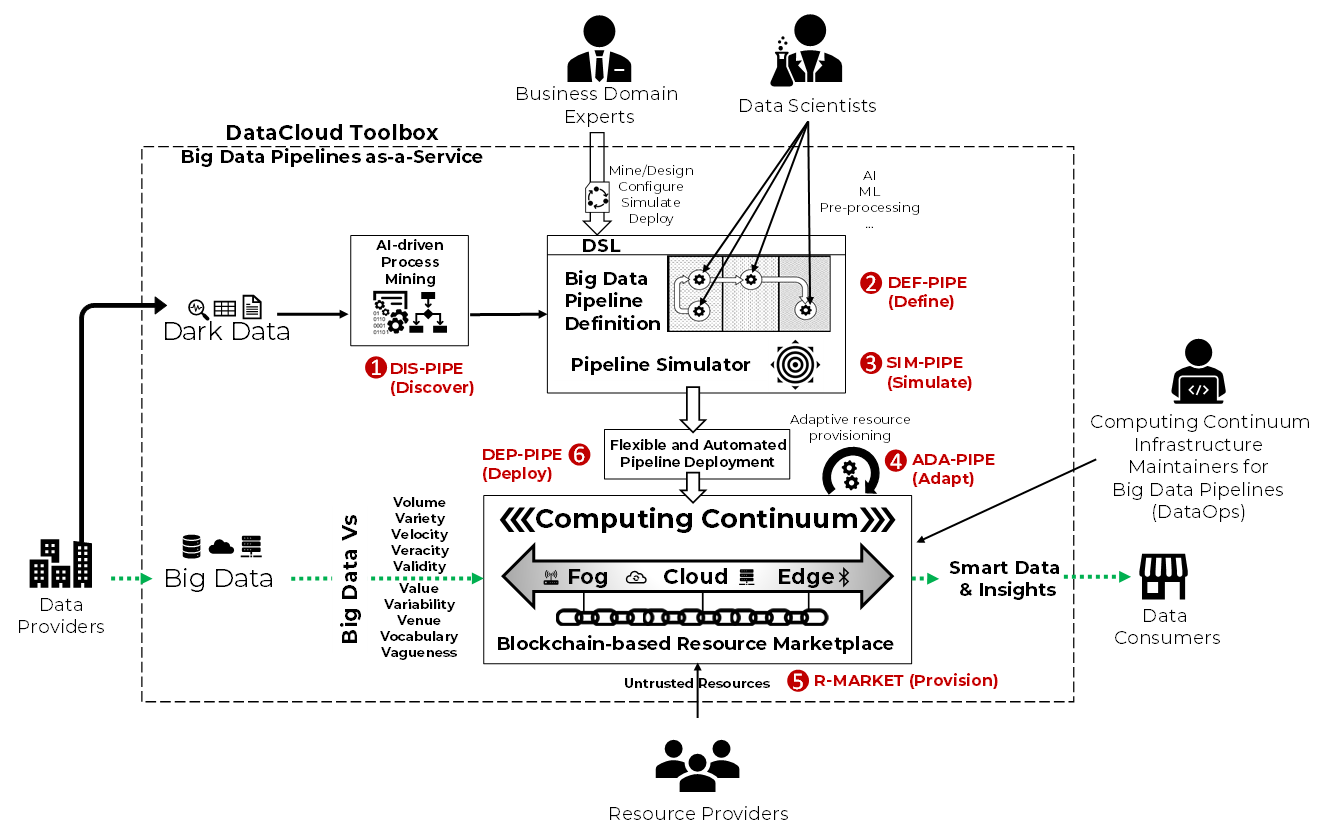
\includegraphics[width=0.95\textwidth]{figures/datacloud_toolbox.png}
                \caption{DataCloud Toolbox Overview \cite{dumitruDataCloudToolbox}}
                \label{fig:datacloud-toolbox-overview}
            \end{figure}
            
            \subsubsection*{DIS-PIPE}
            \label{sec:discover-pipe-datacloud}

                DIS-PIPE (Discover pipeline) \cite{agostinelliDISPIPE2023} uses a set of process mining techniques and AI algorithms to analyse and learn the structure of Big Data pipelines. This is done by extracting, processing and interpreting the vast amount of event data that is collected by multiple heterogeneous data sources. Additionally, the DIS-PIPE module includes a variety of analytics techniques that help to visualise the discovered pipelines together with diagnostics information regarding their execution. 

            \subsubsection*{DEF-PIPE}
            \label{sec:definition-pipe-datacloud}

                DEF-PIPE (Definition pipeline) \cite{mitrovicDEFPIPEFrontend2022} uses domain-specific language (DSL)\footnote{https://www.jetbrains.com/mps/concepts/domain-specific-languages/} to provide a visual design for the implementation of Big Data pipelines.
                This includes support for storing and loading the pipeline definitions and displaying them in a UI. For this, the pipeline structure is declared by domain experts.
                Furthermore, it is designed to allow Data Scientists to define the content by providing the configuration of each pipeline step.

            \subsubsection*{SIM-PIPE}
            \label{sec:simulation-pipe-datacloud}

                The SIM-PIPE (Simulation pipeline) \cite{nikolovSIMPIPE} module generates and simulates a deployment configuration that takes hardware requirements into account and also includes additional middleware information that is required. The generated result is then used for the final deployment.
                The module also includes a sandbox that enables the evaluation of individual pipeline steps to analyse the performance as well as a simulator for determining the performance of the Big Data pipeline.
                
            \subsubsection*{ADA-PIPE}
            \label{sec:adaptation-pipe-datacloud}

                ADA-PIPE (Adaptation pipeline) \cite{mehranADAPIPE2023} is the module that we are working on.
                ADA-PIPE provides a data-aware algorithm for smart and adaptable provisioning of resources and services. The tool allows resource reconfiguration for improved computational performance and interoperability by monitoring and analysis of diverse resources. 
                
                The monitoring of resources and the mapped pipeline tasks allow analysing of the gathered data to be able to make more accurate predictions in the future based on machine learning algorithms that are specifically made for the prediction of time-series or sequential data.

            \subsubsection*{R-MARKET}
            \label{sec:resource-market-datacloud}

                R-MARKET (Resource-MARKET) \cite{senguptaRMARKET} deploys a decentralized resource network that is based on a hybrid of permissioned and permissionless blockchain. This blockchain federates a set of heterogeneous resources from multiple providers spread across the Computing Continuum.
                R-MARKET provides a marketplace for resources at every service layer that is managed in a trustful democratic manner.
                The marketplace enables the provisioning of resources over multiple domains for external use.

            \subsubsection*{DEP-PIPE}
            \label{sec:deploy-pipe-datacloud}

                DEP-PIPE (Deploy-PIPE) \cite{ledakisDEPPIPE} provides elastic and scalable deployment and orchestration of Big Data pipelines while addressing run-time aspects.
                The module also features real-time event detection and automated decision-making for automated deployment and orchestration.

        \subsection{Required REST Interfaces for Collaboration}
        \label{sec:required-interfaces}

            \subsubsection{Pipelines}
            
                \begin{description}
                    \item[Endpoint] \texttt{/pipelines}
                    \item[REST Methods] \texttt{GET, POST}
                    \item[Description] The pipelines endpoint is used to get a JSON file that contains a list of all pipelines that are currently running in the DataCloud system with the \texttt{GET} method. To upload a new pipeline and its tasks, the \texttt{POST} method can be used. The process after posting the pipeline is described in section \ref{sec:requirement-file-preprocessing-server}. Once a pipeline is successfully uploaded using the \texttt{POST} method, it can also be retrieved with the \texttt{GET} method as long as the pipeline is running inside the system.
                \end{description}

                
            \subsubsection{Requirements}

            \begin{description}
                \item[Endpoint] \texttt{/requirements/<pipeline\_id>}
                \item[REST Methods] \texttt{GET}
                \item[Description] This endpoint returns the requirements of each job of the pipeline that is specified with its \texttt{pipeline\_id}. The requirements include parameters such as the maximum resource limits of a task that are not to be exceeded or the docker image and its location. Also included in the requirements are the dependencies of each task to tasks that have to be executed beforehand.
            \end{description}
                
            \subsubsection{Resources}

            \begin{description}
                \item[Endpoint] \texttt{/resources}
                \item[REST Methods] \texttt{GET}
                \item[Description] This endpoint returns a list of all resource providers and their worker pools to the requesting client. The worker pools contain metadata, such as their name, the name of each worker, the number of workers and their resource capabilities. The resource capabilities include values such as the number of virtual CPU cores, and the memory and storage capacity.
            \end{description}

            \subsubsection{Schedules}

            \begin{description}
                \item[Endpoint] \texttt{/schedules/<pipeline\_id>}
                \item[REST Methods] \texttt{GET}
                \item[Description] This endpoint returns a schedule of tasks of a pipeline that corresponds to the identifier \texttt{pipeline\_id}. The tasks are returned in a list that is ordered based on the order they should be deployed on the resources. The tasks contain metadata such as the resource they need to be deployed on, the resource limits that are not to be exceeded for the task as well as the adapted resource utilisation that was predicted via machine learning.
            \end{description}

    \section{Server}
    \label{sec:server}

        This section describes the used third-party tools and concepts used to implement the server of \nameref{sec:adaptation-pipe-datacloud}.
        It was agreed upon by all developers to use \nameref{sec:rest-server} for the communication between the different pipeline components of DataCloud with specific interfaces (see \ref{sec:api-server}) to send messages.

    % todo describe what will be mentioned in this section

        \subsection{REST}
        \label{sec:rest-server}

            REST \cite{redhatWhatRESTAPI} (short for Representational State Transfer) was created for building web services and provides a set of constraints and properties
            that are used to make web services \emph{RESTful}. RESTful web services are built to be scalable, flexible and maintainable.
            REST is based on the HTTP protocol and relies on client-server communication, where a client first sends a request and the server sends back a response.
            The response contains a representation of the requested resource, which is JSON for the ADA-PIPE module.
            The communication between ADA-PIPE and other modules uses \nameref{sec:api-server}s in other to forward or retrieve data.

        \subsection{Application Programming Interface}
        \label{sec:api-server}

            An Application Programming Interface (API) \cite{redhatWhatRESTAPI} is a set of protocols and tools for building software and applications.
            APIs are used to provide endpoints for different software systems (i.e. applications, services, etc.) to communicate and exchange data with each other.
            The communication and interaction of different software components are defined via an API and they also allow these interactions to take place over the internet.
            The required API endpoints to cooperate with other DataCloud pipelines are defined in section \nameref{sec:required-interfaces}.

        \subsection{Flask}
        \label{sec:flask-server}

            Flask \cite{WelcomeFlaskFlask} is a Python framework for creating web applications.
            The main benefit of Flask compared to other web application frameworks for Python like Django is that it is easy and quick to get started, yet scaling up to complex web applications is easily possible and most important a lightweight framework.
            Flask is often used for small to medium-sized projects and is known for its simplicity and ease of use.

            In ADA-PIPE, Flask is used to implement and expose the \nameref{sec:rest-server} server to other components (see \ref{fig:datacloud-toolbox-overview}) of DataCloud via an \nameref{sec:api-server}.

        \subsection{KeyCloak Authentication}
        \label{sec:keycloak-server}

            KeyCloak \cite{keycloakDocumentationKeycloak} is an open-source identity and access management tool.
            DataCloud has decided to use this tool to ensure authenticated communication between all services as well as its users.
            In DataCloud, the possibly sensible data requires to be handled securely, making KeyCloak a feasible tool for user federation and access control. KeyCloak is based on strong standard protocols and provides support for many common communication protocols such as OpenID Connect, OAuth 2.0 and SAML.
            Another major feature of KeyCloak is that it can be used for many popular programming languages such as Java, JavaScript and in our case Python. The KeyCloak library implementation of each language can be used with every other KeyCloak implementation via REST calls and given the distributed working environment and usage of different programming languages depending on the expertise of each team, KeyCloak is a suitable choice for providing authentication and authorization of users and services.

            In DataCloud, the responsibility of providing authentication tokens is done by a KeyCloak server instance.
            In order to be able to communicate with other DataCloud microservices, ADA-PIPE first has to retrieve a KeyCloak authentication token from the server instance. This authentication token is similar to a session key often found for web services and is only valid for a predefined time frame. This authentication token must be sent with every request to other microservices and every microservice inside of DataCloud is required to verify the validity of the sent token.

            In ADA-PIPE, before acquiring the authentication token for our service, an instance of the \emph{KeycloakOpenID} has to be created with the proper credentials, such as \emph{server URL, client id, realm name} and \emph{client secret key}. Since especially the client's secret key has to be concealed, a function is used to load the key into memory so that it can not be easily read. This KeycloakOpenID instance is created as is shown in listing \ref{lst:keycloak-open-id}.
            
            \lstinputlisting[language=Python, caption=Retrieve KeyCloak OpenID Instance, label=lst:keycloak-open-id]{code_samples/kc_open_id.py}
            After successfully creating the KeycloakOpenID instance, the authentication token for ADA-PIPE can be retrieved from the KeyCloak server. This is done by providing the username and password that is used for ADA-PIPE to the method \texttt{\_get\_keycloak\_token(...)} that can be seen in listing \ref{lst:get-keycloak-token}. This method uses the KeycloakOpenID to send the provided credentials to the Keycloak server, and if those are valid, then the server sends back the keycloak token.
            
            \lstinputlisting[language=Python, caption=Get ADA-PIPE KeyCloak Token, label=lst:get-keycloak-token]{code_samples/kc_get_service_token.py}
            After the successful request of acquiring a keycloak token, we can send this keycloak token with each of our requests to other DataCloud services. This is done to authenticate the messages that are sent to other microservices and since each microservice has a unique token that is linked to it, the token is verifiable by a method such as the code in listing \ref{lst:kc-verify-token}, that is used in ADA-PIPE to authenticate incoming messages. This is done by first checking the HTTP status code. If the HTTP status code is \texttt{201 OK}, then the token is valid. Additionally, the response body is checked for the fields \texttt{email\_verified} and \texttt{preferred\_username}. Either of these must be included in the response for the message to be verified by our service. Otherwise we either get a \texttt{4xx} HTTP error status code or reject the message if the required fields are missing in the response.

            \lstinputlisting[language=Python, caption=KeyCloak Token Verification, label=lst:kc-verify-token]{code_samples/kc_token_verification.py}

        \subsection{Processing of Incoming Data}
        \label{sec:processing-of-data-server}

            In this section, the processing of the incoming data will be discussed.
            The incoming data in this scenario is a Big Data task pipeline that should be mapped and then deployed to the resources in the Computing Continuum. The Big Data task pipeline is defined in a custom DSL \cite{mehranDSLDEFPIPEExample2023} that is sent from DEF-PIPE to ADA-PIPE and is then preprocessed before analysing and scheduling the tasks. 

            \subsubsection{Requirement File Structure}
            \label{sec:requirement-file-structure-server}

                As mentioned, the incoming file structure is a custom DSL.
                It is structured similarly to a JSON file with a few distinctions, but the key-value pattern and the nested value sections are similar. At the root level, the keyword \texttt{Pipeline} is always followed by the name of the pipeline.
                At the next nesting level, the keywords are as follows: 
                \begin{itemize}
                    \item \texttt{communicationMedium}, which denotes what type of service the pipeline tasks are, for example, that they consist of a set of web service tasks.
                    \item \texttt{environmentParameters}, which is a set of parameters that are required to interact with the environment such as Kubernetes and other services.
                    \item \texttt{steps}, which is the task pipeline itself that consists of all the tasks. This also includes the dependencies of tasks to other tasks and is usually shown by the order in the tasks mentioned in the pipeline as well as a nested keyword \texttt{previous} that denotes all services that have to be running before the task this keyword resides in. Each step also describes the hardware requirements and how scalable a task has to be.
                \end{itemize}
                

            \subsubsection{Requirement File Preprocessing}
            \label{sec:requirement-file-preprocessing-server}

                Since the incoming data is provided in a DSL scheme, and the next DataCloud module DEP-PIPE is responsible for the deployment of the tasks onto resources expects the file format in a JSON scheme, we parse the incoming data and convert the file as a JSON file. For this, we receive the data via REST and extract the message body and parse it.
                After parsing the JSON message body, the extracted data is stored in Python objects of the classes \texttt{JobDataContainer} and \texttt{PipelineDataContainer}. 
                The \texttt{PipelineDataContainer} class is used to store the data of the entire incoming pipeline, its structure, order and its metadata. It holds the jobs/tasks as \texttt{JobDataContainer} objects that each holds the metadata and properties of the jobs.
                The jobs in the pipeline are stored in a list, that is sorted ascending based on the dependencies upon other tasks.


        \subsection{Testing the Server}
        \label{sec:testing-the-server}

        % todo either merge with subsubsection or find another testing method

            \subsubsection*{Insomnia}
            \label{sec:insomnia-server}
            
                For testing the server REST responses, we use the tool Insomnia \cite{konginc.IntroductionInsomnia}.
                Insomnia is a popular cross-platform REST (Representational State Transfer) client for testing and debugging REST APIs. It allows developers to easily send HTTP requests and view responses, making it an indispensable tool for working with RESTful APIs. Some of the key features of Insomnia include support for multiple request methods (such as GET, POST, PUT, etc.). Insomnia also provides real-time request and response previews, as well as the ability to validate and format JSON data.
                As is already stated, Insomnia stores the requests and is also capable of validating JSON data, and we used this functionality to test the responses of the server for correctness.

                % todo mention unit tests of insomnia
                   

            \subsubsection*{Nmap}
            \label{sec:nmap-server}

                Network Mapper (Nmap) is a popular open-source tool for network discovery and security auditing. It is often used for tasks such as network inventory, monitoring hosts or service uptime as well as looking for vulnerabilities in network components.

                \begin{quote}
                    Nmap uses raw IP packets in novel ways to determine what hosts are available on the network, what services (application name and version) those hosts are offering, what operating systems (and OS versions) they are running, what type of packet filters/firewalls are in use, ... \cite{NmapNetworkMapper}
                \end{quote}

                In ADA-PIPE we use Nmap to test if the network component that provides our REST services (see section \ref{sec:rest-server}) is reachable and also only exposes the necessary ports to do so. Nmap also proves a service to run scripts that look for common vulnerabilities. If a possible vulnerability is found by a script, it gets listed with the corresponding CVE number.
                A found vulnerability in the system was found (see listing \ref{lst:nmap-output}) by Nmap using the command: \texttt{\$ sudo nmap -sV -script=vuln <ip\_number>}. To enable the scripts that look for vulnerabilities, the flag \texttt{-script=vuln} needs to be included. 
                As stated in the Nmap report, the port number \texttt{8011} is vulnerable to a \emph{directory traversal} attack in the \emph{phpMyAdmin} \cite{phpmyadminBringingMySQLWeb} service. The details of the vulnerability can be found with its identifier \texttt{CVE-2005-3299} and also by the references provided by the script.
                

                \lstinputlisting[language=Bash, caption=Nmap Vulnerability Output Example, label=lst:nmap-output]{code_samples/nmap_output.bash}

            % And then we found out that Tinky did a big Stinky and we rejoiced.             

    \section{Monitoring}
    \label{sec:monitoring}

    % todo shortly provide an overview here
            
        \subsection{Netdata}
        \label{sec:netdata-monitoring}

            Netdata \cite{netdataGettingStartedLearn2023} is an open-source tool that collects real-time metrics, including CPU usage, disk activity, bandwidth usage and furthermore.
            The reason we chose Netdata for monitoring is that it is a lightweight tool mostly written in C, Python and Javascript and it requires minimal resources, which is necessary when monitoring edge devices.
            One of its major features is that it runs without interrupting any of the applications running on the same device. This is achieved by only using idle CPU cycles while running.

            Netdata provides an in-browser dashboard to analyse each metric in real-time with help of visual representation. As an example, a screenshot was taken of a cloud resource in our system as can be seen in \ref{fig:netdata-dashboard}.

            \begin{figure}[h!]
                \centering
                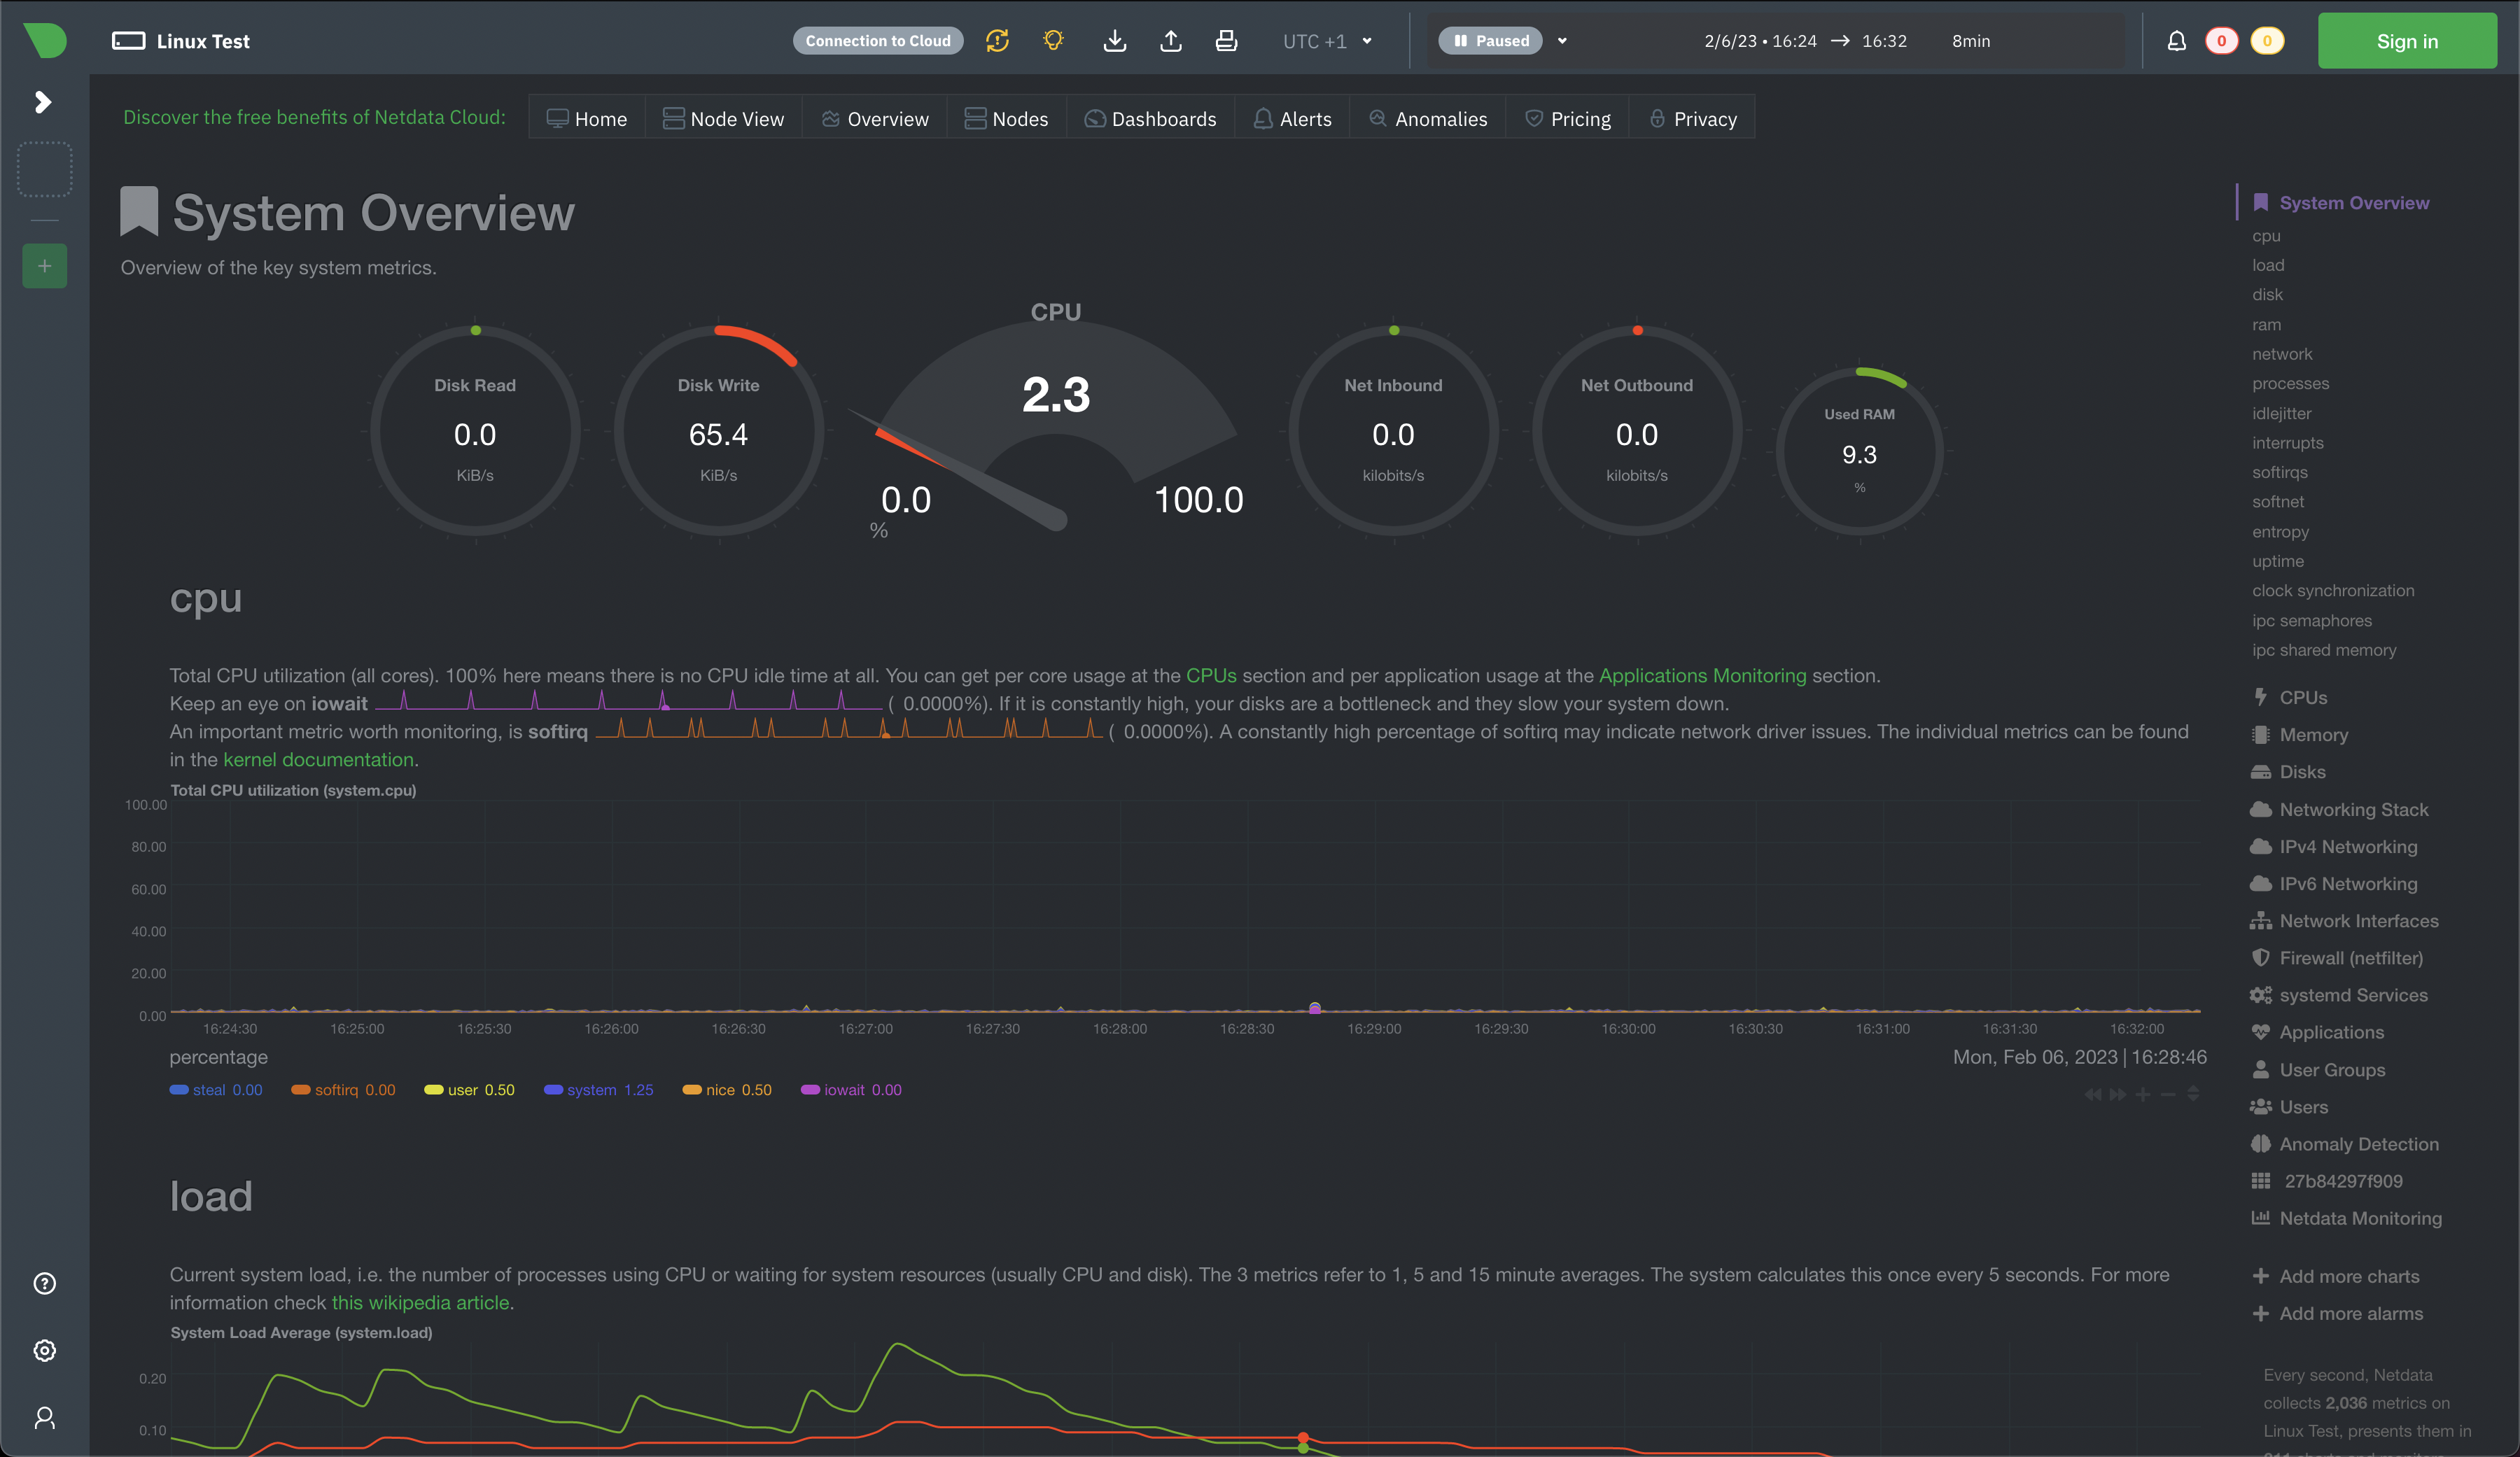
\includegraphics[width=0.95\textwidth]{figures/netdata.png}
                \caption{Netdata Dashboard Example}
                \label{fig:netdata-dashboard}
            \end{figure}
            Netdata has a vast amount of support for other tools in order to gather data. 
            One of the supported tools is \nameref{sec:prometheus-monitoring}, which is used to scrape the monitored data from all resources that have Netdata installed.


        \subsection{Prometheus}
        \label{sec:prometheus-monitoring}
            Prometheus \cite{prometheusOverviewPrometheus} is an open-source application used for monitoring and alerting events and is designed to run across various platforms in a scalable and easily deployable manner.
            Same as Netdata it records in real-time, and stores the gathered metrics in a time series database by using a \emph{HTTP pull model}. It also allows real-time alerting via a rule-defining configuration and also has a flexible query language called \emph{PromQL}, that enables the retrieval and processing of the gathered data. Prometheus has great integration with other tools such as Netdata.
            In the project, it is used inside a monitoring master node that is continuously scraping all resources that have Netdata installed for monitoring data. In case a predefined rule is broken at a monitored resource, such as CPU over-allocation, Prometheus triggers an event that notifies ADA-PIPE in order to be able to take measurements.
            

    \section{Project Planning}
    \label{sec:project-planning}

        The internal project planning was done with Skype Business\footnote{https://www.skype.com} and Trello\footnote{https://trello.com}.
        Skype is used as a video communication tool to discuss the current progress of the project and the future steps to take.
        Trello is a project management tool that uses boards and cards to organize tasks among all members.
        We organized our Trello board similar to a Kanban board and assigned the tasks according to the previous discussions on Skype.
        
        For project steps that are important for other stakeholders of DataCloud, the ADA-PIPE GitHub project board is used similarly to the Trello board. This is done to ensure others see the current tasks of the team members as well as the ones that are already done or are in the backlog. Also, they can add tasks to the project board, such as bugs to be fixed or missing API functionality.
        
    \section{Code Quality}
    \label{sec:code-quality}

    % todo add an overview description to this section

        \subsection{Code Review}
        \label{sec:code-review-code-quality}

        Code reviews are an important part of software development and have several key tasks:
        \begin{itemize}

            \item \textbf{Improving code quality:} Code reviews help ensure that the code is well-written, follows best practices and standards, and is free of bugs or potential security issues.
            
            \item \textbf{Sharing knowledge:} Code reviews are a way for team members to learn from each other and share their expertise and knowledge.

            \item \textbf{Enhancing team collaboration:} Code reviews encourage collaboration and teamwork among team members, helping to foster a positive and inclusive work environment.

            \item \textbf{Maintaining consistency:} Code reviews help ensure that code is consistent and follows the project's style guide and coding standards.

            \item \textbf{Enhancing documentation:} Code reviews can help identify areas where documentation needs to be improved and encourage developers to add more detail and clarity to their code.

            \item \textbf{Finding and fixing bugs:} Code reviews can help identify and fix bugs before they make it into production, reducing the need for bug fixing in the future.

            \item \textbf{Improving performance:} Code reviews can help identify areas where code performance can be improved, helping to ensure that the application is running optimally.

            \item \textbf{Enhancing maintainability:} Code reviews can help ensure that the code is maintainable and easy to understand, making it easier to make changes and upgrades in the future.

        \end{itemize}
            Therefore, a code review of each commit by a collaborator is a healthy process to make sure that each member of the team is aware of the key components of a module.
            This is ensured by using \emph{Pull Requests} on GitHub, where the project resides. In this, a (squashed) commit is only merged into the development branch after at least one other team member has reviewed the code and deemed it acceptable to be included in the project.
            This process is done to ensure that coding conventions are kept consistent\footnote{For this project, the Python coding convention PEP8 is used and enforced. See \url{https://peps.python.org/pep-0008/}} with the existing code base, to ensure an overview understanding of the code base of all members and to quickly find code sections that need improvement or could lead to an erroneous behaviour.

    \subsection{Code Refactoring}
    \label{sec:code-refactoring-code-quality}

        Code refactoring of pre-existing code was necessary in order to be able to use the components with other modules of the project.
        The reason for this is that many functionalities were written in Python scripts that were not written to be included with other modules at that stage.
        % \begin{quote}
        %     Code refactoring is defined as the process of restructuring computer code without changing or adding to its external behavior and functionality. 
        % \end{quote}
        Therefore, the functionality of the scripts was analysed and then put in separate methods.
        Hardcoded sections of the scripts were put into variables or abstracted were possible. 
        Since most of the hardcoded sections were specific file paths that were manually changed depending on which functionality was tested, those hardcoded sections were exported to configuration YAML files to be able to add further configuration files to the project.


    \subsection{Type Hinting and Linting}
    \label{sec:type-hinting-code-quality}

        Python supports \emph{type hinting}\footnote{https://docs.python.org/3/library/typing.html} since version 3.5.
        This enables type annotation for functions, variables and other components.
        Note that type hinting is not enforced and can only be used to declare a type of a code section, but even then, it is not checked nor analysed by the Python runtime.
        Yet, correctly using type hinting enhances the code readability and even makes the method documentation section of each parameter and its type unnecessary in trivial cases. Also, it enables other users to easily use the methods and classes since all its parameters and fields are annotated with the corresponding type.

        As an example of the usage of type hinting in the project, the \texttt{PipelineState} class constructor is shown in the following listing:
        \lstinputlisting[language=Python, caption=PipelineState Constructor, label=lst:pipeline-init]{code_samples/pipeline_init.py}
        Type hints for variables and parameters are denoted with the syntax \texttt{<variable\_name> ":" <type>}.
        There is also the variant of \texttt{<method\_signature()> "->" <type>}, that denotes the return type of a method.
        The return type of the function in listing \ref{lst:pipeline-init} is \texttt{None}, meaning it does not return a value.

        A major benefit of using type hinting not mentioned above is that \emph{Linters} use the provided type hints to enable type checks before runtime. 
        In short, a linter is a tool to improve the written code. Linters diagnose the code and warn about technical issues, inconsistent coding style, security and performance issues. This helps to omit using the wrong data types even in an interpreted programming language such as Python in many cases as we get a warning if a type is used that was not hinted at by us.
        What makes linter tools a valuable addition to the used tool set, and in the project, the linter \emph{PyLance}\footnote{https://marketplace.visualstudio.com/items?itemName=ms-python.vscode-pylance} is used. 

        
    \section{Future Work}
    \label{sec:future-work}

    % todo add short overview of future work

        % \subsection{Concurrency}
        \subsection{Extensive Documentation}
            Documentation is available to some extent in the current version of the project, yet lacks documentation for many sections, such as an overview of the overall system, and the installation guide for new users.
            For this, we will use GitHub wiki functionality that enables us to provide documentation for the project next to the GitHub repository.
            
        \subsection{Swagger}
            % chatGPT
            Swagger is an open-source software framework used for designing, building, and documenting RESTful APIs. It provides a way for developers to describe the structure of their APIs, including the inputs and outputs, and to generate interactive documentation and client libraries in different programming languages. Swagger allows for the creation of APIs that are easily readable and accessible, making it easier for developers to understand how to interact with an API. The Swagger framework also provides tools for testing and validating APIs, allowing developers to quickly identify and fix any issues. The use of Swagger has become a standard for documenting and describing RESTful APIs, making it easier for developers to build and consume these APIs.
            While Swagger is already in use, it only covers parts of the REST API and project.



        \subsection{Server Load Testing}

    % chatGPT
        Server load testing is the process of evaluating the performance of a server under a simulated heavy load. This involves simulating a high number of users or requests to the server to see how it performs under stress. The purpose of server load testing is to identify any performance bottlenecks or limitations before the server is deployed in a production environment so that any necessary improvements can be made to ensure that the server can handle the expected traffic and load. The results of server load testing can be used to optimize the server's configuration, identify and fix any scalability issues, and improve the overall performance of the server.


    \bibliographystyle{ieeetr}
    \bibliography{references}
\end{document}

